\documentclass[9pt,conference,twocolumn]{IEEEtran}

%\usepackage{pdfsync}
%\usepackage{epsfig}
\usepackage{boxedminipage}
%\usepackage{multirow}
\usepackage{amsmath}
\usepackage{comment}
\usepackage{cite}
%\linespread{1.3}
%\usepackage{times}
%\usepackage[sort]{natbib}
\usepackage{graphicx}

\newcommand{\squishlist}{
   \begin{list}{$\bullet$}
    { \setlength{\itemsep}{0pt}      \setlength{\parsep}{0pt}
      \setlength{\topsep}{3pt}       \setlength{\partopsep}{0pt}
      \setlength{\listparindent}{-2pt}
      \setlength{\itemindent}{-5pt}
      %\setlength{\itemindent}{10pt}
      \setlength{\leftmargin}{1em} \setlength{\labelwidth}{0em}
      \setlength{\labelsep}{0.5em} } }

\newcommand{\squishlistindent}{
   \begin{list}{$\bullet$}
    { \setlength{\itemsep}{0pt}      \setlength{\parsep}{0pt}
      \setlength{\topsep}{3pt}       \setlength{\partopsep}{0pt}
      \setlength{\listparindent}{-2pt}
      %\setlength{\itemindent}{-5pt}
      \setlength{\itemindent}{20pt}
      \setlength{\leftmargin}{1em} \setlength{\labelwidth}{0em}
      \setlength{\labelsep}{0.5em} } }

\newcommand{\squishend}{
    \end{list}  }




\begin{document}

\title{Cost-Effective Integration of Three-Dimensional (3D) ICs Emphasizing Testing Cost Analysis}
\maketitle

\begin{abstract}
With conventional memory technologies approaching their scaling limit,
emerging non-volatile memory technologies have attracted increasing%considerable
attention because of their non-volatility, high access speed, low power
consumption, and good scalability. Resistive RAM (ReRAM), with its simple
structure, small cell size ($4F^2$), and the support for 3D stacking, has been
a promising candidate among emerging memory technologies.
A key advantage of ReRAM
comes from its non-linear nature, which enables  cross-point
RAM array structures without having a dedicated access transistor for each cell. While
cross-point design is effective in improving the memory density, it has
inherent disadvantages which introduce extra design challenges. Based on
the device characteristics, we propose a
mathematical model to perform a comprehensive analysis of issues of
reliability, energy consumption, and area overhead for the cross-point array structure. In addition to the
cell-level analysis, different programming schemes are also discussed in
this paper. The proposed model enables designers to identify the most
energy/area efficient ReRAM organization and cell parameters that meet
specific design goals during the early design stage.
\end{abstract}

%\vspace{10pt}
\section{Introduction}\label{sec:intro}
The scaling of traditional memory technologies, such as DRAM and FLASH, is
approaching its physical limit. In the past few years, emerging
non-volatile memory technologies~(NVM), such as Phase Change RAM~(PCRAM),
Spin-transfer-torque RAM~(STT-RAM), and Resistive RAM~(ReRAM) have been
widely studied as potential candidates for the next generation memory
technologies to meet the requirement of higher density, faster access
time, and lower power consumption. Among all of these emerging memory
technologies, ReRAM has many unique characteristics, including simple
structure, non-linearity,  and high resistance ratio, making itself one of
the most promising technologies. Researchers have shown that the
state-of-the-art single-level-cell ReRAM can achieve $7.2ns$ random access
time for both read and write operations with a resistance ratio larger
than 100~\cite{ReRAM_ISSCC2011_Sheu}. Also, HP labs and Hynix have already
announced plans to commercialize memristor-based ReRAM and predicted
that ReRAM could eventually replace traditional memory
technologies~\cite{memristor:HpHynix}.

Unlike other non-volatile memory technologies, ReRAM can be implemented in
a cross-point style structure without any access device. Specifically, in
a nano cross-point array, each bistable ReRAM cell is sandwiched by two
orthogonal nanowires. Thus the area occupied by each cell is $4F^2$ per
bit. However, the simplicity of the access-device-free, cross-point
structure introduces challenges to the peripheral circuit and memory
organization design.

While there have been prior studies on cross-point ReRAM
arrays~\cite{crossbar_NANO2002_Ziegler,crossbar_NANO08_Flocke,crossbar_TED_2010,crossbar_NANO2003_Ziegler},
they do not consider the effect of voltage drivers and programming methods
on the array. In addition, detailed area and energy analysis is also
absent. In this work, we address the design challenges of cross-point
structure based ReRAM. We build an accurate mathematical model to evaluate
memory reliability, energy consumption, and area overhead for different
designs and cell parameters. The advantages of nonlinearity $K_r$ and
write current $I_w$ scaling are all discussed in detail. Our study allows
for exploring the most energy/area efficient ReRAM design with different
design constraints and cell parameters at the very beginning of the design
stage. Moreover, system designers can also leverage the proposed
model to provide valuable feedback to device researchers who will in turn
adjust ReRAM cell design. We believe that this kind of collaboration will
be very helpful to shorten the time to market of ReRAM memory.

The rest of this paper is organized as follows. In
Section~\ref{sec:preliminary}, an overview of ReRAM technology and
cross-point architectures is given. Section~\ref{sec:model} % Section~III
discusses the proposed mathematical model for the cross-point structure
ReRAM and the edge conditions for different write and read schemes.
Section~\ref{sec:w_and_r} analyzes different design constraints of write
and read operations on cross-point based ReRAM arrays. The energy
consumption and area overheads are also analyzed in this section. Then in
Section~\ref{sec:scale}, the effect of nonlinearity and write current on
the design constraints is evaluated. Finally, the conclusion is presented
in Section~\ref{sec:conclusion}.

%\vspace{10pt}
\section{Related Work}\label{sec:related}
 
%\vspace{10pt}
\section{Modeling of the Cross-Point Memory}\label{sec:model}

%In this section, we present a detailed mathematical model for cross-point
%arrays. By using this model, along with specific parameters and edge
%conditions, the reliability, energy consumption, and area overheads of
%different read/write schemes can be easily evaluated.

%\subsection{Basic model of Cross-Point Memory}
The basic circuit model of an $M$ by $N$ cross-point ReRAM array is shown
in Figure~\ref{fig:modeling}. The model is built upon Kirchhoff's Current
Law (KCL) and its validity can be guaranteed by deductions from the basic
circuit theory. The horizontal lines are wordlines and vertical lines
represent bitlines. The ReRAM cells are located at each cross-point of
wordline and bitlines. The resistance of the ReRAM cell at the cross-point
of $i^{th}$ wordline and $j^{th}$ bitline is represented by $R_{i,j}$. We
assume the resistance of the wire connecting two cross-points to be
$R_{line}$. The input resistance of each wordline and bitline is $R_v$ and
the resistance of sense amplifier is $R_s$. In order to set up the KCL
equations, the voltage at each cross-point is indicated as $V_{i,j}$ for
wordline and $V'_{i,j}$ for bitline. A detailed cross-point is also shown
in Figure~\ref{fig:modeling}(b). The input voltage for the $i^{th}$
wordline is $V_{Wi}$ and the $i^{th}$ bitline is $V_{Bi}$. In the case
where a wordline takes input from both the sides, the voltage at the other
end of the $i^{th}$ wordline is represented as $V'_{Wi}$.
%Finally, the voltage at the sense amplifier is $V'_{Bi}$ during the read operation.
%YOU MIGHT WANT TO CHANGE THE ABOVE PARA INTO A TABLE

\begin{figure}%[!hb]
\centering
  % Requires \usepackage{graphicx}
  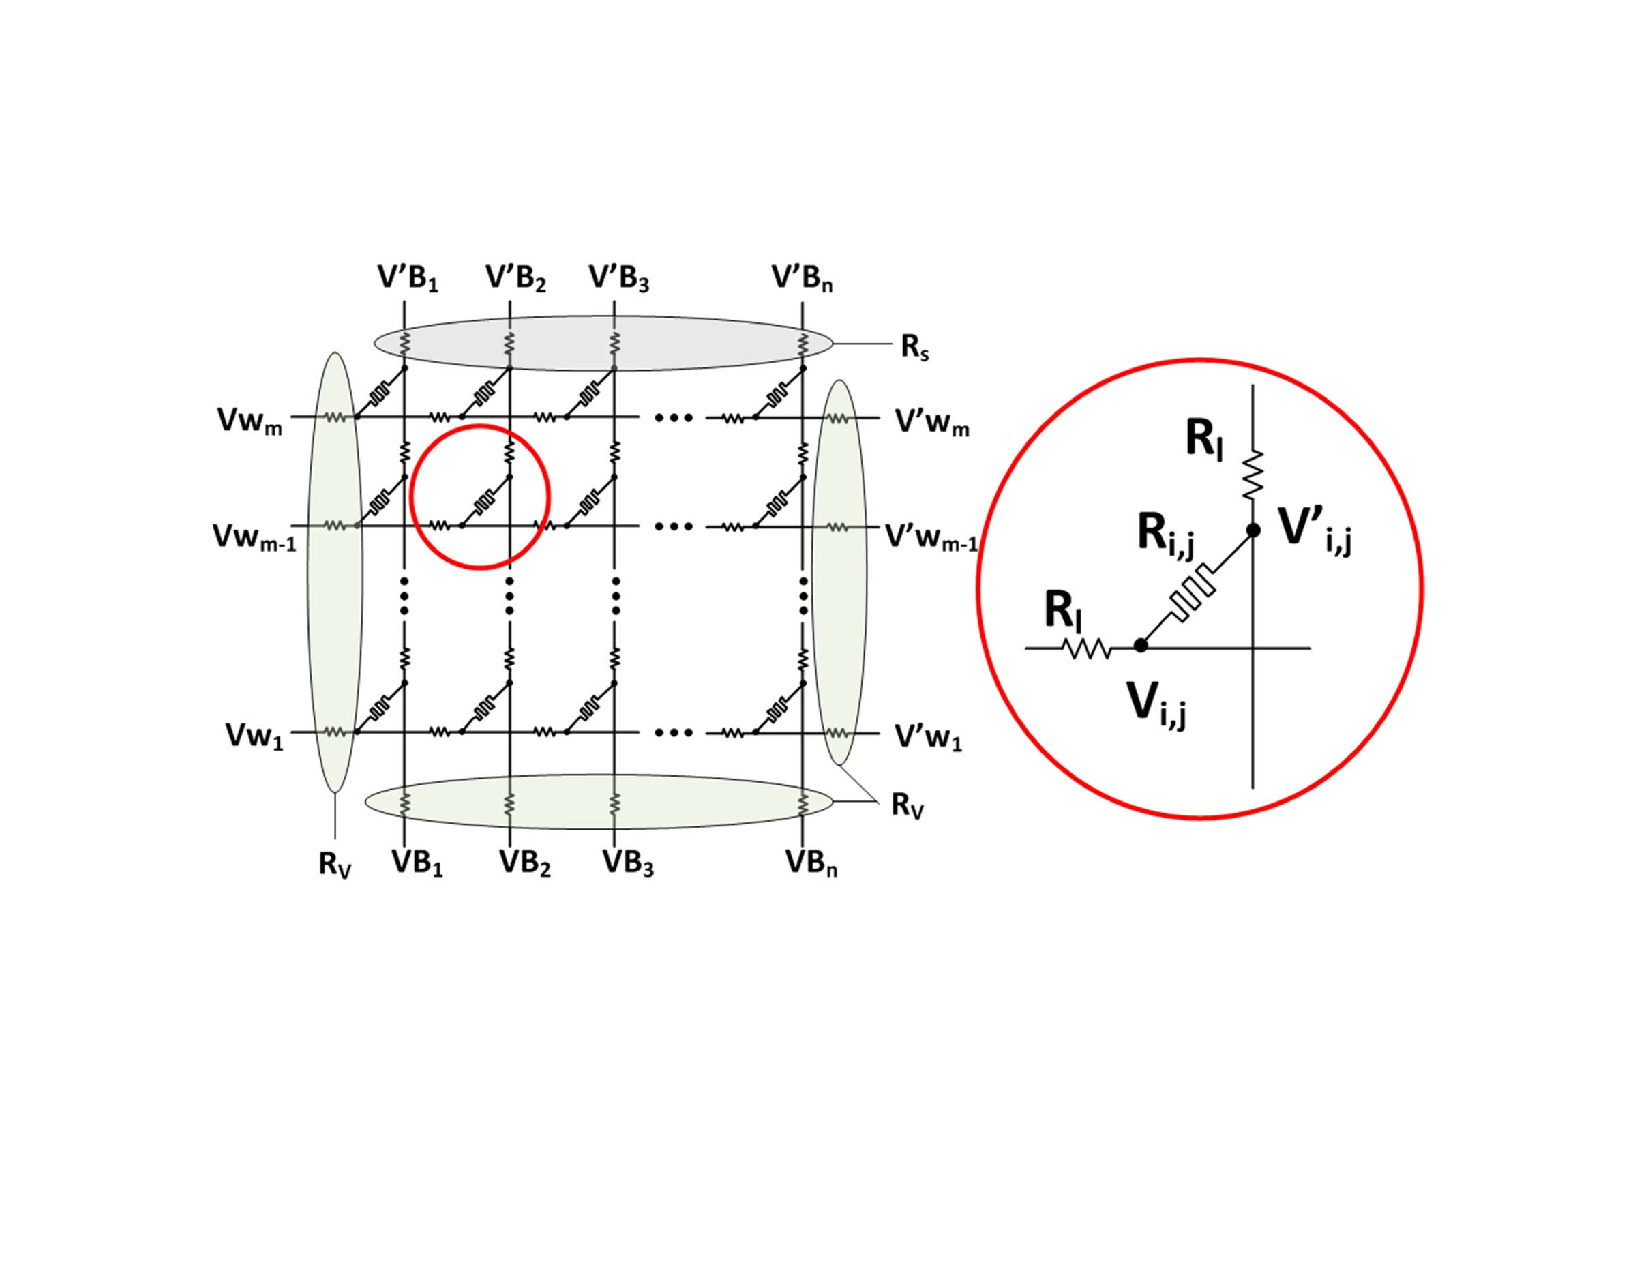
\includegraphics[width=0.45\textwidth]{./figures/model_f.pdf}\\
  \caption{The basic model of typical cross-point array.}\label{fig:modeling}
  \vspace{-12pt}
\end{figure}

%\subsection{Mathematical Model of a Cross-Point Array}
Based on this model, the current equations for each cross-point can be set
following KCL: $ {\Sigma}_{I=1}^kI_k=0.$ All of the cross-points have
similar structure with no more than three current branches and therefore
it is very easy to set up the KCL equations for each cross-point. However,
we should treat the cross-points at the edges of the array specifically
because KCL equations for these cross-points vary with different
write/read schemes. For example, the unselected wordline for write
operation can be either half biased or left floating. Thus, the edge
conditions should be adjusted according to each write/read scheme. In
particular, all of the cross-points in an array can be classified into
three major categories: \emph{normal point}, \emph{activated point} and
\emph{floating point}.

The normal points are located inside the memory array. In other words, for
all of the nodes with $1<i<m$ and $1<j<n$, the KCL equations take the form
of
\begin{equation}\label{equ:KCL1}
R_l^{-1}V_{i,j-1} -(2R_l^{-1}+R_{i,j}^{-1})V_{i,j}+ R_l^{-1}V_{i,j+1}+R_{i,j}^{-1}V'_{i,j}=0,
\end{equation}
for the node at wordline layer and
\begin{equation}\label{equ:KCL2}
R_l^{-1}V'_{i-1,j} -(2R_l^{-1}+R_{i,j}^{-1})V'_{i,j}+ R_l^{-1}V'_{i+1,j}+R_{i,j}^{-1}V_{i,j}=0,
\end{equation}
for the node at bitline layer.

The activated point and floating point represent the nodes at the edge of
cross-point array with different conditions: an edge point, which is
directly connected to the voltage input or to the ground, can be
considered as an activated point. Otherwise, it is a floating point. For
example, consider the point located at the intersection of $i^{th}$
wordline and $1^{st}$ bitline. If the $i^{th}$ wordline is activated by an
input voltage of $V_{Wi}$, this cross-point is an activated point, and the
KCL equation for this point is:
\begin{equation}\label{equ:KCL3}
-(R_v^{-1}+R_l^{-1}+R_{i,1}^{-1})V_{i,1}+ R_l^{-1}V_{i,2}+R_{i,1}^{-1}V'_{i,1}=-R_v^{-1}V_{Wi}.
\end{equation}
Otherwise, it is floating and its KCL equation is
\begin{equation}\label{equ:KCL4}
-(R_l^{-1}+R_{i,1}^{-1})V_{i,1}+ R_l^{-1}V_{i,2}+R_{i,1}^{-1}V'_{i,1}=0.
\end{equation}

For clarity, a ${2mn\times 1}$ vector ${V}$ is defined to represent all of the variables in the KCL equations:
\begin{equation}\label{equ:V1}
{V}=[{V_1}^T,{V_2}^T...{V_m}^T,{V'_1}^T,{V'_2}^T...{V'_m}^T]^T,
\end{equation}
where,
%\begin{equation}\label{equ:V2}
%{V_i} = [V_{i,1},V_{i,2}...V_{i,n}]^T,\\
%\end{equation}
%\begin{equation}\label{equ:V3}
%{V'_i} = [V'_{i,1},V'_{i,2}...V'_{i,n}]^T,
%\end{equation}
\begin{equation}\label{equ:V2}
{V_i} = [V_{i,1},V_{i,2}...V_{i,n}]^T,~~{V'_i} = [V'_{i,1},V'_{i,2}...V'_{i,n}]^T,
\end{equation}
for $i=1,2...m$. Then all of the KCL equations can be considered as a
system of linear equations, which has the form
\begin{equation}\label{equ:matrix}
A\cdot V = C.
\end{equation}
$A$ is a ${2mn\times{2mn}}$ coefficient matrix, which is determined by
Equations(\ref{equ:KCL1})-(\ref{equ:KCL4}). $C$ is a ${2mn\times{1}}$
vector, containing the constant terms of these equations. As shown, all of
the KCL equations have simple structure and are similar to each
other. Therefore, the linear equation system has a relatively fixed format
and simple structure, making it easy to establish and adjust the
coefficients and constants according to different design schemes. Besides,
due to the simplicity of the KCL equation, $A$ is populated primarily with
zeros and can be saved as a sparse matrix, which will further reduce the
storage cost during the computation.

To validate our analytical model, we compared the results with the HSPICE
simulations using a simple resistor model in cross-point memory arrays. DC
analysis was performed by HSPICE which solved the voltage of every node in
the array. The results of eight cross-point arrays with different array
size and specific data pattern are shown in Figure ??, the voltage drop on
the selected cell derived from our analytical model are consistent with the
HSPICE simulation results.
\begin{figure}%[!t]
\centering\label{fig:SPICE}
  % Requires \usepackage{graphicx}
  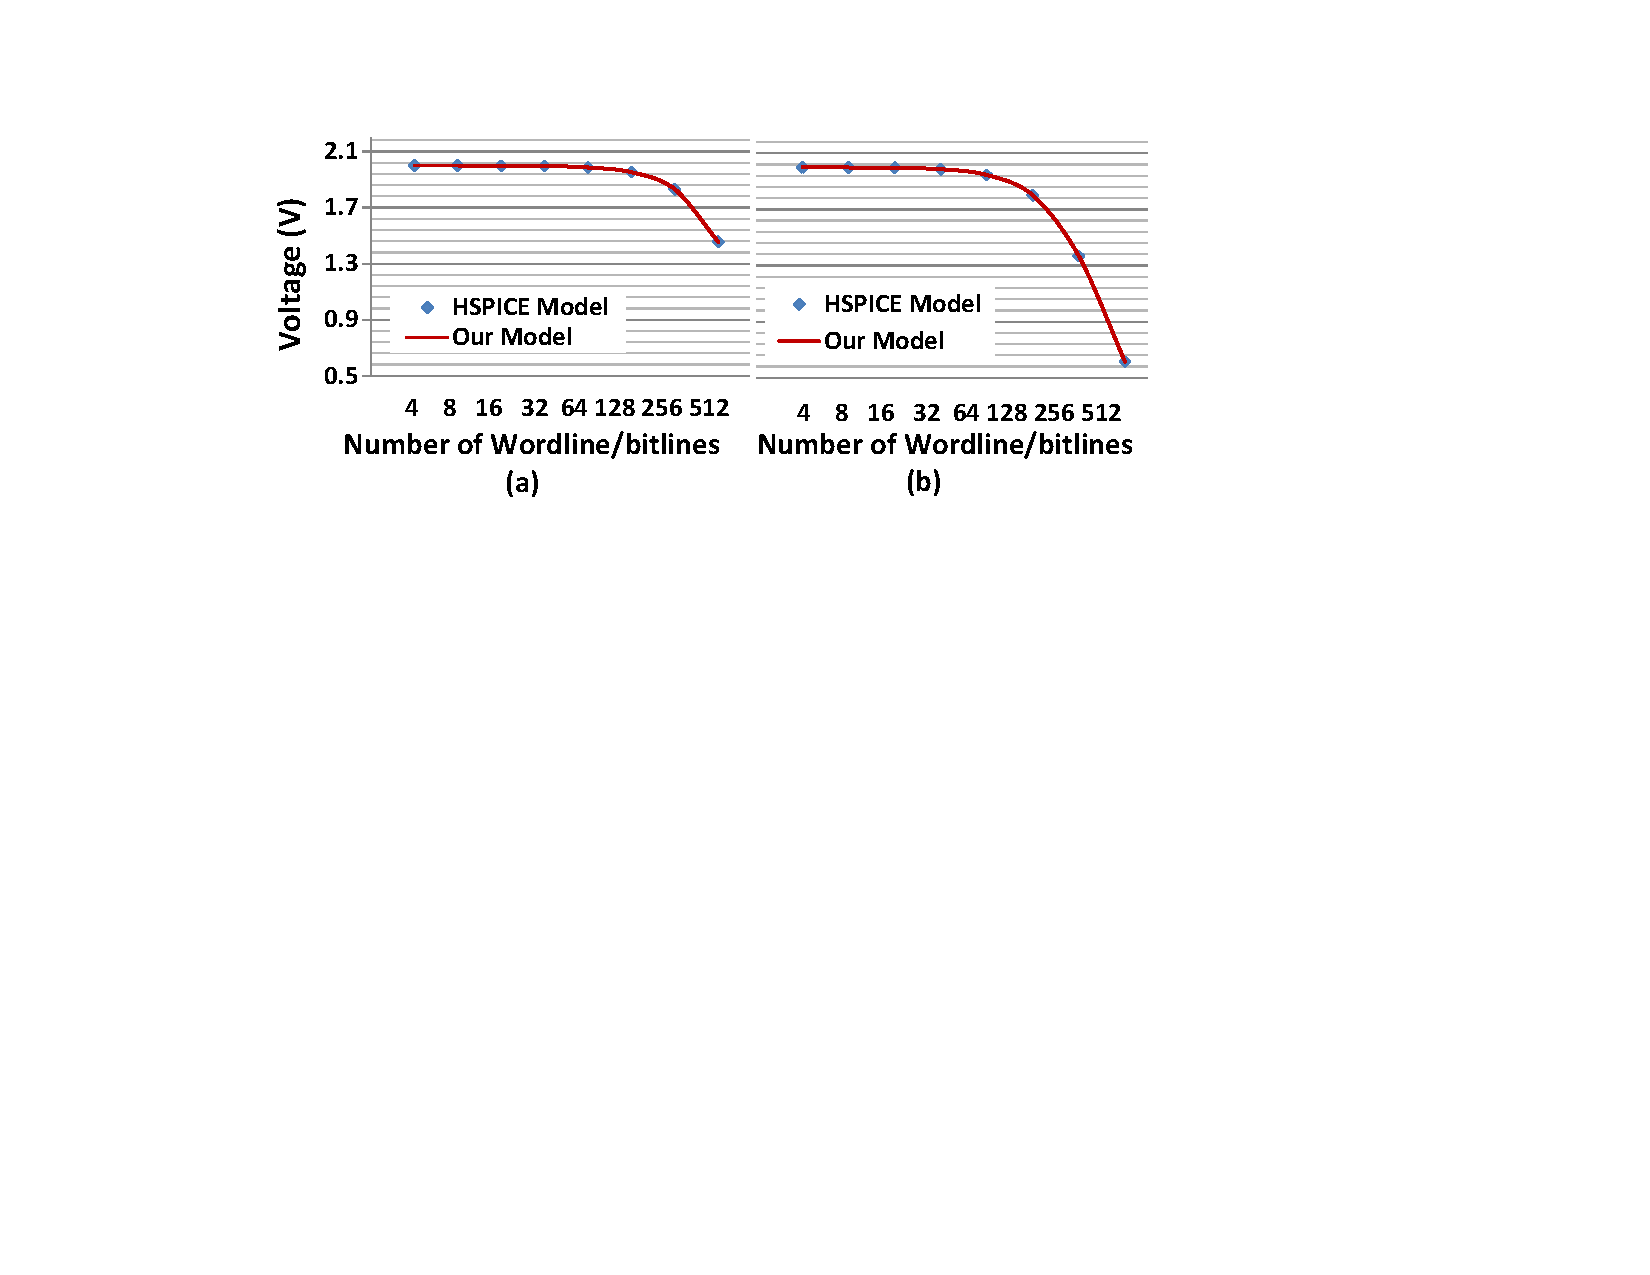
\includegraphics[width=0.5\textwidth]{./figures/SPICE.pdf}\\
  \caption{Analytical model verification of voltage drop comparing to HSPICE simulations (a) with non-linearity of 5; (b) without non-linearity.}\label{fig:reliable_region}
    \vspace{-10pt}
\end{figure}
%
%The characteristics of the linear system can be summarized as:
%\begin{enumerate}
%  \item
%  As shown in Equation~(\ref{equ:blockedmatrix}), the coefficient matrix $A$ can be further partitioned into 4 smaller subblocks :
%    \begin{equation}\label{equ:blockedmatrix}
%        \mathbf{A} = \left[
%        \begin{array}{cc}
%            A1 & A2  \\
%            A3 & A4  \\
%        \end{array} \right].
%    \end{equation}
%All of these subblocks have the same size of $m\times n$. Subblock
%$A2$ and $A3$ are diagonal matrixes and have the value of: $A2_{i,i} =
%A3_{i,i} = R_{i,i}^{-1}$. $A2$ and $A3$ do not change their values
%with different schemas. However, $A1$ and $A4$ are a little more
%complex than $A2$ and $A3$. $A1$ is a tridiagonal matrix and has
%nonzero elements only in the main diagonal, and the first line below
%and above the diagonal. Similarly, $A_4$ is a special tridiagonal
%matrix, which has nonzero elements in the main diagonal, and the
%$n^{th}$ line below and above the diagonal, where $n$ is the number of
%bitline in the cross-point model. The value of the elements in $A1$
%and $A4$ can be easily derived from Equation (\ref{equ:KCL1}) and
%(\ref{equ:KCL2}). However, the edge condition varies with different
%program schemes. Therefore, the coefficients related to the edge
%condition should be set according to the program schemes. Clearly, the
%four edges shown in Figure~\ref{fig:modeling} correspond to different
%coefficients in $A1$ and $A4$. Due to the space limitations, we
%consider the nodes at the left edge of the array as an example. A
%similar procedure can be followed to initiate the coefficients of
%other edge. The coefficients of nodes at the left edge of the array
%($V_{i,1}$) can be set as:
%
%    \begin{equation}
%    A1(k,k) = \left\{
%    \begin{array}{ll}
%    -(R_l^{-1}+R_{i,1}^{-1})   & \text{if } floating\\
%    -(R_v^{-1}+R_l^{-1}+R_{i,1}^{-1})& \text{if } activated
%    \end{array} \right.
%    \end{equation}
%    where $k=(n-1)i+1$ for $i=1,2...m$.
%
%  \item The constant terms $C$ is a $2mn{\times}1$ vector. Equation(\ref{equ:KCL1})-(\ref{equ:KCL4}) show that only KCL equations of the activated points have constant terms. Therefore, only the following elements in $C$ may have non-zero value: $C((i-1)n+1)$, $C(in)$, $C(mn+i)$ and $C((2m-1)n+i)$ for $i=1,2...m$, corresponding to the nodes at the four edges respectively. Likewise, as an example, we consider nodes $V_{i,1}$. The constant corresponding to these nodes can be defined as:
%    \begin{equation}
%    C((i-1)n+1) = \left\{
%    \begin{array}{ll}
%    0   & \text{if } floating\\
%    -R_v^{-1}V_{Wi}& \text{if } activated
%    \end{array} \right.
%    \end{equation}
%\end{enumerate}
Thus, with parameters such as the resistance of ReRAM cells, the
resistance of interconnect wires, program voltages, and write/read
schemes, voltages at various cross points can be obtained by solving the
system of linear equations. With detailed voltage values,
$V_{2mn{\times}1}$, we can analyze the array at a fine granularity. These
values are also critical to evaluate reliability, energy consumption,
driven current density, and area overheads of a cross-point array.

\input{analysis}
%\input{prediction}
\input{space}

\bibliographystyle{ieeetran}
\bibliography{./bib/crossbar,./bib/memristor}

\end{document} 